\documentclass{standalone}
\usepackage{amsmath}
\usepackage{amssymb}
\usepackage{tikz}
\usepackage{mathrsfs}
\usepackage{ifthen}

\newcommand{\perpp}{\perp\!\!\!\perp}
\DeclareMathOperator{\so}{\mathfrak{s}}
\DeclareMathOperator{\ra}{\mathfrak{r}}
\DeclareMathOperator{\supp}{supp}
\DeclareMathOperator{\id}{id}
\DeclareMathOperator{\dom}{dom}
\DeclareMathOperator{\ran}{ran}
\DeclareMathOperator{\Min}{Min}
\DeclareMathOperator{\cod}{cod}
\newcommand{\smallerthan}{<}
\newcommand{\greaterthan}{>}
\newcommand{\defeq}{:=}
\newcommand{\eqdef}{=:}

\newcommand{\cat}[1]{\textbf{#1}}
\DeclareMathOperator{\IG}{\mathscr{IG}}


\begin{document}
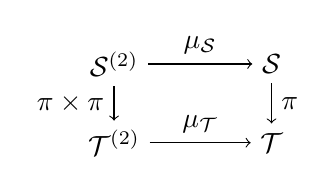
\begin{tikzpicture}
    \node (S2) at (0,0) {$\mathcal{S}^{(2)}$};
    \node (S) at ([shift={+(2,0)}]S2) {$\mathcal{S}$};
    \node (T2) at ([shift={+(0,-1)}]S2) {$\mathcal{T}^{(2)}$};
    \node (T) at ([shift={+(2,0)}]T2) {$\mathcal{T}$};
    \draw[->] (S2)--(S) node[midway,above] {$\mu_{\mathcal{S}}$};
    \draw[->] (S2)--(T2) node[midway,left] {$\pi\times\pi$};
    \draw[->] (S)--(T) node[midway,right] {$\pi$};
    \draw[->] (T2)--(T) node[midway,above] {$\mu_{\mathcal{T}}$};
    

\end{tikzpicture}\end{document}